% !TEX TS-program = XeLaTeX
\documentclass[a4paper]{article}

\input{lang}

% https://tex.stackexchange.com/a/5365
% Must
\usepackage[table]{xcolor}

\usepackage{tabularx}


\usepackage{tikz}
\usepackage{fontspec,lipsum}
%\usepackage{color}
\usepackage{color,colortbl}

\definecolor{Gray}{gray}{0.9}

% https://tex.stackexchange.com/questions/172234/define-and-set-length-in-one-command
\newcommand{\deflen}[2]{%      
    \expandafter\newlength\csname #1\endcsname
    \expandafter\setlength\csname #1\endcsname{#2}%
}

\newcommand{\goldenratio}{1.618}

% Page margins
%\deflen{verticalmarg}{\dimexpr(\goldenratio\horizontalmarg)}
\deflen{verticalmarg}{0.7cm}
\deflen{horizontalmarg}{\dimexpr(\verticalmarg)}

\usepackage[top=\the\verticalmarg, bottom=\the\verticalmarg, 
  left=\the\horizontalmarg, right=\the\horizontalmarg]{geometry}


\deflen{lowerbaroffset}{0.8cm}

\deflen{contentswidth}{\dimexpr(\paperwidth-2\horizontalmarg)}
\deflen{contentsheight}{\dimexpr(\paperheight-2.01\verticalmarg)}

\deflen{halfwidth}{\dimexpr(0.6\contentswidth)}


\deflen{paramarg}{0.25cm}

\deflen{colwidth}{\dimexpr(\halfwidth-\paramarg)}

\deflen{lowersectionstart}{\dimexpr(0.56\contentsheight)}
\deflen{headermarg}{2cm}

%% The vertical lines at which things should align
\deflen{haligni}{0cm}
\deflen{halignii}{\colwidth}
\deflen{haligniii}{\dimexpr(\halfwidth+\paramarg)}
\deflen{colwidthr}{\dimexpr(\contentswidth-\haligniii)}
\deflen{haligniv}{\dimexpr(\contentswidth)}


%% Horizontal lines at which things should align
\deflen{valigni}{\contentsheight}
\deflen{valignii}{\dimexpr(\contentsheight-\headermarg)}
\deflen{valigniii}{\lowersectionstart}
\deflen{valigniv}{\dimexpr(\lowersectionstart-\headermarg)}


%% TODO: If we just need two columns, maybe it is better to use a style for that
%% rather than laying out the columns ourselves using Tikz.

% A paragraph: Args (X, Y, text)
\newcommand{\anemoparagraph}[4]{
  \node[anchor=north west,style={inner sep=0,outer sep=0}] at (#1,#2) {
    \begin{minipage}[l]{#3}
      #4
    \end{minipage}
  };
}

%% TODO: Can easily convert USD or EUR

\newcounter{cumulativechf}

\newcommand{\resetchf}{\setcounter{cumulativechf}{0}}
\newcommand{\chf}[1]{
  #1 CHF
  \addtocounter{cumulativechf}{#1}
}

% Draw a vertical bar across the contents area
\newcommand{\vhelper}[1]{\draw[color=gray] (#1,0cm) -- (#1,\the\contentsheight);}

% Draw a horizontal bar across the contents area
\newcommand{\hhelper}[1]{\draw[color=gray] (0cm,#1) -- (\the\contentswidth,#1);}

% Display helper lines
\newcommand{\helpers}{
  \draw[color=gray] (0,0) rectangle (\the\contentswidth, \the\contentsheight);
  \vhelper{\the\halignii}
  \vhelper{\the\haligniii}
  \hhelper{\the\valignii}
  \hhelper{\the\valigniii}
  \hhelper{\the\valigniv}
}

% A4: 21.0 × 29.7
\pagenumbering{gobble}
\newcommand{\usefontmuli}{\setmainfont[Path=../fonts/]{Muli-Regular.ttf}}
\newcommand{\usefontboing}{\setmainfont[Path=../fonts/]{BoingBold.otf}}

\usefontmuli

% (x, y, contents)
\newcommand{\mainheader}[3]{
  \usefontboing
  \node[anchor=north west] at (#1,#2) {\Huge #3};
  \usefontmuli
}



\definecolor{Anemored}{RGB}{255, 33, 63}


% https://tex.stackexchange.com/a/159576
\newcommand{\HRule}[1][\medskipamount]{\par
  \vspace*{\dimexpr-\parskip-\baselineskip+#1}
  \noindent\rule{\linewidth}{0.2mm}\par
  \vspace*{\dimexpr-\parskip-.5\baselineskip+#1}}

% To be used inside a column
% contents
\newcommand{\subheader}[1]{
  \color{Anemored}
  \begin{flushleft}
    \large #1
  \end{flushleft}
  %\noindent\rule{\the\colwidth}{0.4pt}
  \HRule[-0.1cm]
  \vspace{0.5cm}
  \color{black}
}


% A two-column table suitable for specs
% Alternating colours
\newcommand{\spectable}[2]{
  \renewcommand{\arraystretch}{1.4}
  #1 \\
  \begin{tabularx}{\colwidthr}{X X}
    \hline #2
  \end{tabularx}\vspace{0.3cm}
}

% TODO: See if Melissa provided some design document
% with precise specs of margins, font sizes, etc.


\newcommand{\textfield}[1]{
  \fboxrule=0.4pt
  \fbox{
    \begin{minipage}[t][1cm][t]{0.95\colwidth}
      \textbf{#1}
    \end{minipage}
  }
}



%% Page on how to make rotated headers
%% and check marks, just what we want
%% for the feature list:
%% https://tex.stackexchange.com/a/98439
\usepackage{pifont}
\newcommand*\rot{\rotatebox{90}}
\newcommand*\OK{\ding{51}}

% Table headers
\newcommand{\tabh}[1]{\textbf{#1}}
\newcommand{\roth}[1]{\rot{\textbf{#1}}}

\begin{document}
\noindent
\begin{tikzpicture}[x=1cm, y=1cm]
\definecolor{anemored}{rgb} {1.00,0.129,0.247}

\small

% Helper lines
%\helpers
\mainheader{\the\haligni}{\the\valigni}{\enfr{Anemomind Plans}{Plans Anemomind}}
\anemoparagraph{\the\haligni}{\the\valignii}{\the\colwidth}{
  \large
  \subheader{\enfr{The Anemobox}{L'Anemobox}}
  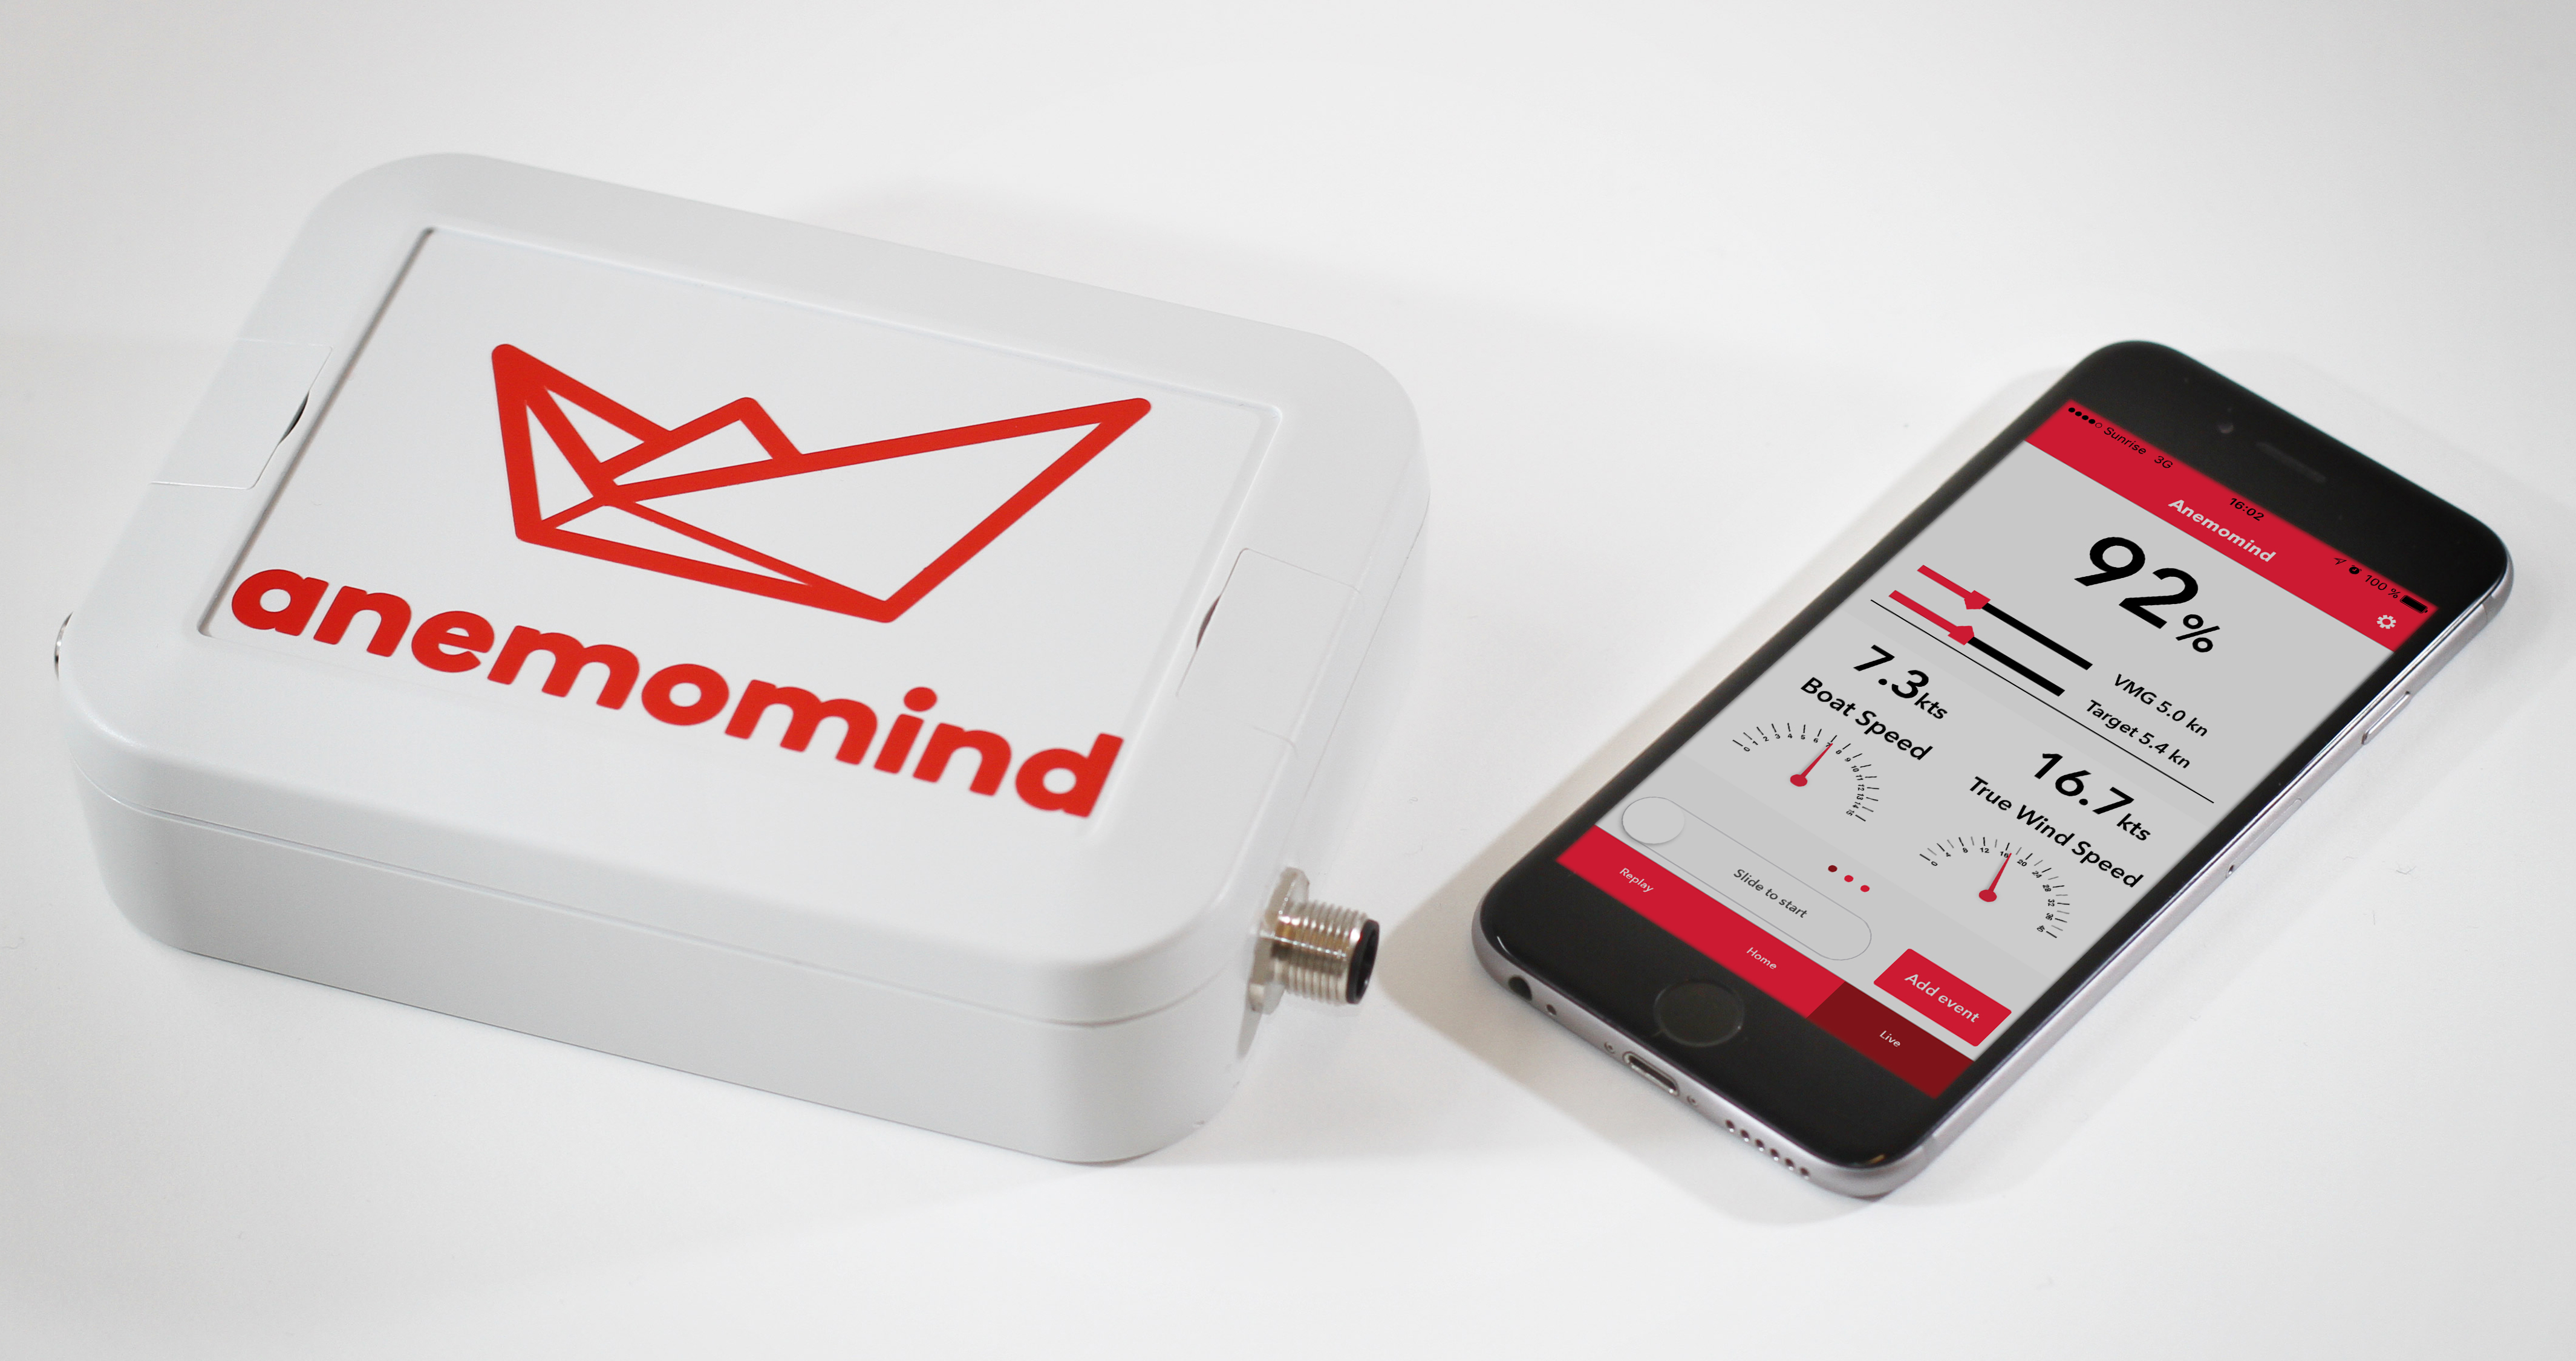
\includegraphics[width=\the\colwidth]{../images/anemobox10.jpg}
  \enfr{The Anemobox is the heart of the Anemomind system. It is a small onboard computer that captures data from sensors via NMEA. Those data are recorded to log files for deep analysis but also available in real-time via WiFi on your tablet or phone.}{L'Anemobox est le c\oe ur de la système Anemomind. C'est une petite ordinateur abord qui capture les données des senseurs par NMEA. Ces données sont enregistrées sur des fichiers log pour une analyse profonde mais aussi affichées en temps réelle par WiFi sur ta tablette ou smartphone.}
}

\anemoparagraph{\the\haligniii}{\the\valigniv}{\the\colwidthr}{
  \subheader{\enfr{Subscription Plans}{Plans de souscription}}

  \bigskip
      {
        \renewcommand{\arraystretch}{2}
        \begin{tabularx}{\colwidthr}{|X|c|c|c|}
          \cline{2-4} % https://tex.stackexchange.com/a/64827 : Remove certain borders
          \multicolumn{1}{c|}{} & \roth{Social sailors} & \roth{Amateur racers} & \roth{Professional racers } \\ \hline
          \enfr{Public navigation sharing}{Partage navigations publique} & \OK & \OK & \OK \\ \hline
          \enfr{Unlimited navigation data storage}{Espace illimité de données navigation} & \OK & \OK & \OK \\ \hline
          \enfr{Performance estimation}{Estimation pérformance} & & \OK & \OK \\ \hline
          \enfr{Full instrument display}{Affichage d'instruments} & & \OK & \OK \\ \hline
          \enfr{VMG table}{Tableau VMG} & & \OK & \OK \\ \hline
          \enfr{Private sharing with team}{Partage privé avec équipe} & & & \OK \\ \hline
          \enfr{Raw data export (CSV)}{Export données bruts (CSV)} & & & \OK \\ \hline
        \end{tabularx}
      }
}


%% https://www.senero-marine.ch/wp-content/uploads/2017/01/BandG_Preisliste_2017.pdf
\anemoparagraph{\the\haligni}{\the\valigniv}{\the\colwidth}{
  \subheader{\enfr{Prices}{Les prix}}
  \includegraphics[width=\textwidth]{\enfr{../priceflowen.eps}{../priceflowfr.eps}}
}

\node[anchor=south east,style={inner sep=0,outer sep=0}] at (\the\contentswidth,0cm) {
  \begin{minipage}[l]{3.5cm}
    
\includegraphics[width=\textwidth]{../images/logosmall.pdf}
  \end{minipage}
};

\newcommand{\gigabytes}{\enfr{GB}{Go}}

\anemoparagraph{\the\haligniii}{\the\valignii}{\the\colwidthr}{
  \subheader{\enfr{Anemobox Specs}{Spécs Anemobox}}
  %\rowcolors{2}{gray!25}{white}
  {
    \scriptsize
    \spectable{\enfr{Embedded sensors}{Senseurs embarquées}}{
      \enfr{GPS networks}{Réseaux GPS} & multi-GNSS (GPS/QZSS, GLONASS \enfr{and}{et} BeiDou) \\
      \enfr{GPS accuracy}{GPS qualité mésures} & 2.5 m CEP \\ %% Comment traduire accuracy?
      \enfr{GPS Frequency}{Fréquence GPS} & 1-10 Hz \\
      \enfr{External GPS connectivity}{Connectivitée GPS externe} & NMEA 0183 \enfr{and}{et} 2000 \\
      \enfr{Inertial Measurement Unit}{Centrale inertielle} &	9 axis, 1 kHz \\
      \enfr{Compass}{Compas} & 3 axis magnetometer, \enfr{compensated with}{compensé par} 3 gyroscopes \\
    }
    \spectable{\enfr{Processing Characteristics}{Caractèristiques traitement}}{
      \enfr{Processing}{Traitement} & dual-core, dual-threaded Intel® Atom CPU \enfr{at}{de} 500 MHz \\
      RAM & 1 \gigabytes \\
      \enfr{Logging storage}{Espace fichiers log} & 8 \gigabytes \\
      \enfr{System storage}{Espace système} & 4 \gigabytes \\
    }
\newcommand{\inputoutput}{\enfr{input}{entré} + \enfr{output}{sorti}}
    \spectable{Connections}{
      \enfr{Wireless}{Sans fil} & Wifi, Bluetooth 4.0 \\
      8-poles IP67 \enfr{connector}{connecteur} & \enfr{Power}{Alimentation}, NMEA \inputoutput \\
      NMEA 2000 \enfr{connector}{connecteur} & \enfr{Power}{Alimentation}, data \inputoutput \\
    }
    \spectable{\enfr{Physical Characteristics}{Caractèristiques physiques}}{
      \enfr{Size}{Taille} & 11 $\times$ 15 $\times$ 4 cm \\
      \enfr{Weight}{Poids} & 227 g \\
    }
    \spectable{\enfr{Electrical Characteristics}{Caractèristiques éléctriques}}{
      \enfr{Supply voltage}{Tension alimentation} & 9--24 V DC \\
      \enfr{Power consumption}{Consommation} & 1.5 W \\
      \enfr{Current at}{Courrant à} 12 V & 0.12 A \\
    }
  }
  \rowcolors{2}{white}{white}
}
\end{tikzpicture}
\end{document} 

